
\subsection*{task 2.4 \\[1ex] superpixels (part 2)}

Instead of working with the \emph{mean} intensity value in each $m \times n$ tile of an image, we can also pixelize by using \emph{median} intensities.

Implement a function \keyword{medianSuperPixel} simply by replacing \keyword{np.mean()} in \keyword{meanSuperPixelV2} with \keyword{np.median()}.

For $(m, n) \in \bigl\{ (4,4), (32,32), (16,32), (32,16) \bigr\}$, run \keyword{meanSuperPixelV2} and \keyword{medianSuperPixel} on \texttt{portrait.png} and paste your results here \\[1cm]
%%%%%
%%%%%
%%%%% enter your result here, i.e. replace "placeholder.pdf" by the names of your resulting image files
%%%%%
%%%%%
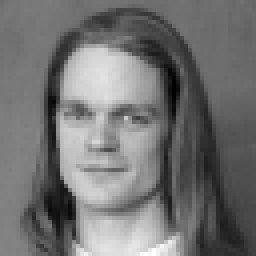
\includegraphics[width=0.24\textwidth]{t4-mean(4, 4).png} \hfill

\includegraphics[width=0.24\textwidth]{t4-mean(32, 32).png} \hfill

\includegraphics[width=0.24\textwidth]{t4-mean(16, 32).png} \hfill

\includegraphics[width=0.24\textwidth]{t4-mean(32, 16).png} 

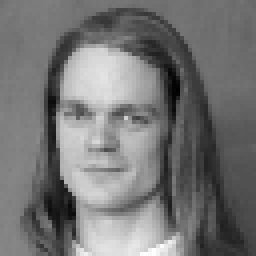
\includegraphics[width=0.24\textwidth]{t4-median(4, 4).png} \hfill

\includegraphics[width=0.24\textwidth]{t4-median(32, 32).png} \hfill

\includegraphics[width=0.24\textwidth]{t4-median(16, 32).png} \hfill

\includegraphics[width=0.24\textwidth]{t4-median(32, 16).png} 
%%%%%
%%%%%
%%%%%
%%%%%
%%%%%





